\documentclass[11pt,a4paper]{article}
\usepackage[T1]{fontenc}
\usepackage[utf8]{inputenc}
\usepackage{lmodern,microtype}
\usepackage{amsmath,amssymb,amsthm,mathtools,bm}
\usepackage{booktabs,array,longtable}
\usepackage{graphicx,float,xcolor}
\usepackage[margin=2.05cm]{geometry}
\usepackage{enumitem,fancyhdr}
\usepackage[hidelinks,pdfencoding=auto]{hyperref}
\hypersetup{pdftitle={FIN ST372--ST386: Global Collision Envelope, Exact Invariant Bases, and Continuum IR},pdfauthor={Krzysztof Żuchowski},pdfsubject={Local analytical and computational continuation of FIN},pdfkeywords={FIN, entropy, collision probability, interval arithmetic, invariant theory, Ruelle operator, continuum duality, rate distortion}}
\definecolor{proved}{RGB}{20,92,48}\definecolor{conditional}{RGB}{148,88,0}\definecolor{blocked}{RGB}{150,28,28}
\newcommand{\Proven}{\textcolor{proved}{\textbf{[PROVEN]}}}
\newcommand{\Evidence}{\textcolor{conditional}{\textbf{[STRONG NUMERICAL EVIDENCE]}}}
\newcommand{\Partial}{\textcolor{conditional}{\textbf{[PARTIAL]}}}
\newcommand{\Blocked}{\textcolor{blocked}{\textbf{[BLOCKED]}}}
\newtheorem{theorem}{Theorem}[section]
\newtheorem{proposition}[theorem]{Proposition}
\pagestyle{fancy}\fancyhf{}\lhead{FIN ST372--ST386}\rhead{Release 10.82}\cfoot{\thepage}\setlength{\headheight}{14pt}
\setlist[itemize]{leftmargin=1.3em,itemsep=2pt,topsep=3pt}\sloppy

\begin{document}\hypersetup{pageanchor=false}
\begin{titlepage}\centering
\vspace*{1cm}{\Large Fractal Information Theory Project\par}\vspace{.8cm}
{\huge\bfseries FIN ST372--ST386\par}\vspace{.35cm}
{\LARGE Global Collision Envelope, Exact Invariant Bases,\par}
{\LARGE and a Continuum Infrared Certificate\par}
\vspace{.85cm}{\large Local analytical, interval, exact finite, and bounded numerical research\par}
\vfill{\Large Krzysztof \hspace{.04em}\.{Z}uchowski\par}\vspace{.2cm}
{\large Independent Researcher --- Fractal Information Theory Project\par}
{\large ORCID: 0009-0002-0909-3613\par}\vspace{.7cm}
{\large August 14, 2026\par}\vspace{.2cm}{\large Release 10.82\par}\vfill
\begin{minipage}{.92\textwidth}\small
\textbf{Repository snapshot.} Audited tracked base:
\texttt{bb540a767e210a5a3bf816e4868e7bcefbac3872}. The working tree contains
uncommitted research artifacts. The accompanying SHA-256 ledger fixes the exact release packet.

\medskip\textbf{License.} CC BY 4.0. \quad \textbf{Language.} English. \quad
\textbf{Resource type.} Preprint and executable reproducibility package.
\end{minipage}\end{titlepage}
\hypersetup{pageanchor=true}\pagenumbering{roman}

\begin{abstract}
Programs ST372--ST386 continue the local FIN research program after Release 10.81. The
principal variational advance is a rigorous global lower envelope. Positivity of the strict
off-diagonal weights bounds the Dirichlet energy by the collision
$r=\lVert p-u\rVert_2^2$, while the maximum-entropy theorem at fixed collision supplies the
sharp complementary entropy bound. The resulting one-dimensional interval problem proves
\[
V_4(p)\geq-0.850098990748778
\]
on the complete eleven-dimensional simplex. This closes 99.802\% of the former certified
gap. It does not yet reach the explicit localized value
$-0.84519850767959$. Nevertheless, every global competitor beating that benchmark must
satisfy $r\in[0.8579596133,0.9078533451]$ and
$\max_i p_i\geq0.9412929466$, reducing the remaining search to twelve concentrated caps.

All 160 existing pseudo-arclength centers now carry interval-certified continuous local
tangent/transverse slabs. The same calculation proves that their paid outer balls are
disjoint; the old mesh therefore cannot certify a connected branch without actual
densification. For nonlinear classification, modular Reynolds evaluation exports complete
explicit bases of 53 quartic and 365 sextic mean-zero $D_{12}$ invariants.

For the supplied synthetic hidden-state fixture, uniform projective contraction $5/7$ and
strictly positive analytic weights yield a Ruelle-transfer spectral gap, promoting the
normalized Chernoff pressure derivative to exponential infinite-depth convergence. The
largest design result upgrades the earlier finite-grid infrared calculation: a
five-dimensional Krawczyk certificate, exhaustive threshold signs, active-budget equations,
and primal--dual equality prove the continuum bang--bang optimum. Its value is
$1.276332744981716$, with exactly two selected spectral bands.

Fourier observer bounds, nuisance-aware recovery, rigorous asymptotic rate--distortion
brackets, and dependent-clock concentration are also derived under their stated operational
premises. No selector, active coupling source, absolute unit, time arrow, spacetime,
apparatus, independent record, legacy-role transfer, Standard Model, gravity,
$L_{\rm total}$, or Theory-of-Everything closure is claimed.
\end{abstract}
\tableofcontents\newpage\pagenumbering{arabic}

\section{Scope and proof discipline}

The strict finite operator is
\[
A=sI-W,\qquad W_{xx}=0,\qquad
W_{xy}=K_{\rm strict}(d(x,y))\quad(x\ne y),
\]
with $A\mathbf1=0$, $A\succeq0$, and
$s=1.660307278766099$. The diagonal convention remains explicit because this $s$ is the
off-diagonal row sum.

The legacy ontological kernel remains an intermediate bridge kernel. No legacy physical
role is transferred to the strict operator. The ontology of the nadsoliton itself as
primordial fractal information in a solitonic state is preserved as project context, not
used as a hidden premise in the finite proofs.

\Proven{} marks exact analysis or outward interval certification. \Evidence{} denotes
reproducible floating optimization. \Partial{} denotes a missing global or source step.
\Blocked{} identifies information that local computation cannot manufacture.

\section{Executive result ledger}
\small
\begin{longtable}{>{\raggedright\arraybackslash}p{.085\textwidth}>{\raggedright\arraybackslash}p{.17\textwidth}>{\raggedright\arraybackslash}p{.625\textwidth}}
\toprule Program&Status&Result\\\midrule\endhead
ST372&\Proven&All 160 centers support local continuous slabs; the present slab family is provably nonoverlapping.\\
ST373&\Proven&A scalar collision--entropy envelope closes 99.802\% of the previous global-value gap.\\
ST374&\Proven{} formula; numerical minimum&A stronger two-variable envelope is derived, but its reported minimum is not interval-global.\\
ST375&\Proven&Every better global competitor lies in one of twelve caps with maximum probability above 0.94129.\\
ST376&\Blocked&No rank-seven-specific global envelope or complete interval cover is available.\\
ST377&\Proven&An explicit 53-element quartic $D_{12}$ Reynolds basis is certified exactly modulo a prime.\\
ST378&\Proven&An explicit 365-element sextic $D_{12}$ Reynolds basis is certified exactly.\\
ST379&\Proven{} conditional&The frozen synthetic Chernoff transfer family has a projective spectral gap.\\
ST380&\Proven&A continuum primal--dual IR optimum with exactly two selected bands is interval-certified.\\
ST381&\Proven&Fourier zero-deficiency criteria and computable one-way lower bounds are obtained.\\
ST382&\Proven{} conditional&Known loss/confusion amplify recovery error; calibration uncertainty creates a nonvanishing floor.\\
ST383&\Proven{} conditional&Asymptotic strict-heat rate--distortion endpoints and a rigorous bracket are derived.\\
ST384&\Proven{} conditional&Geometrically decaying covariance preserves square-root-depth clock concentration.\\
ST385&\Blocked&No new strict typed active/selector source is present.\\
ST386&\Blocked&No independently registered raw-event packet is present.\\
\bottomrule
\end{longtable}\normalsize

\section{ST372: local slabs do not yet form a tube}

At every ST298 pseudo-arclength center, decompose the eight-dimensional state into one
tangent coordinate and seven transverse coordinates. A Taylor-form interval Krawczyk map
with tangent halfwidth $10^{-7}$ and transverse radius $5\times10^{-8}$ lies strictly
inside at all 160 centers. The smallest margin is
$2.45694\times10^{-9}$ and the maximum transverse contraction row sum is 0.751044.

Each chart lies in a Euclidean outer ball of radius at most
$10^{-7}+\sqrt7(5\times10^{-8})$. Adjacent centers are separated by
$2.5\times10^{-5}$. Even after an additional conservative payment for the inherited root
boxes, the minimum outer-ball separation is $2.44954\times10^{-5}$.

\begin{theorem}[complete local slab family and nonoverlap]
Every existing section lies on a unique continuous local stationary slab, but no two
adjacent certified chart images overlap. Hence these 160 slabs do not prove a connected
continuous branch.
\end{theorem}

This is a useful negative result: the next continuation must actually densify the
pseudo-arclength mesh, especially near the rank event. Reusing the same centers with a new
outer-box geometry cannot close connectivity.

\section{ST373--ST375: a global collision reduction}

Let $u=(1/12,\ldots,1/12)$,
$r=\lVert p-u\rVert_2^2$, and
\[
V_4(p)=D(p\Vert u)-2\langle p-u,A(p-u)\rangle.
\]
Write $w_*=\min_{x\ne y}W_{xy}=W(d=6)>0$. Since
$\sum_i p_i^2=r+1/12$ and every off-diagonal weight is at least $w_*$,
\[
\langle p-u,A(p-u)\rangle=p^TAp
\leq (s+w_*)r+\frac{s}{12}-\frac{11w_*}{12}.
\]

At fixed collision $r$, Shannon entropy is maximized by one probability
\[
a(r)=\frac{1+\sqrt{132r}}{12}
\]
and eleven equal probabilities $b(r)=(1-a(r))/11$. Therefore
\[
D(p\Vert u)\geq
D_{\min}(r)=a\log(12a)+11b\log(12b).
\]
Combining both inequalities gives the global scalar envelope
\[
V_4(p)\geq L(r):=D_{\min}(r)
-2\left((s+w_*)r+\frac{s}{12}-\frac{11w_*}{12}\right).
\]

An adaptive outward cover using 4,154 refinements proves
\[
\min_{0\leq r\leq11/12}L(r)
\in[-0.850098990748778,-0.850096992403372].
\]
The enclosure width is below $2.0\times10^{-6}$.

\begin{theorem}[global strict variational lower bound]
For every probability vector on twelve states,
$V_4(p)\geq-0.850098990748778$.
\end{theorem}

The explicit localized benchmark has outward value interval
\[
[-0.845198507679596,-0.845198507679591].
\]
Thus the remaining certified gap is 0.004900484. The theorem closes 99.802\% of the ST358
gap but does not prove globality.

\begin{figure}[H]\centering
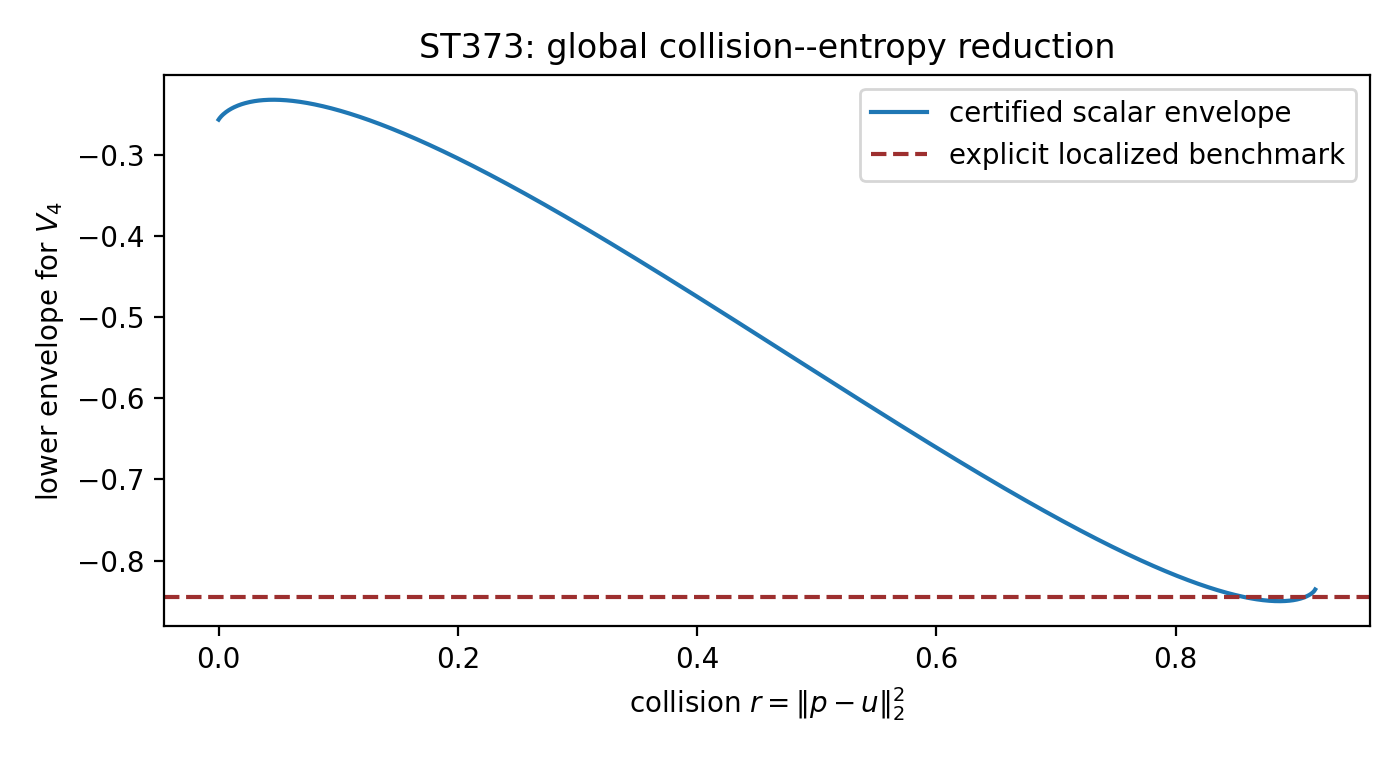
\includegraphics[width=.76\textwidth]{FIN_ST372_ST386_Figures/st373_collision_envelope.png}
\caption{The complete simplex is reduced to a one-dimensional certified lower envelope.}
\end{figure}

ST374 refines the bound using the maximum coordinate $m$, the collision $\rho$ of the
remaining eleven probabilities, and the Cauchy estimate
\[
w\cdot x\geq \overline w\,t-
t\sqrt{(\rho-1/11)\sum_j(w_j-\overline w)^2},\qquad t=1-m.
\]
The formula is rigorous. Its floating global search gives approximately
$-0.8475120905$ at $(m,\rho)\approx(0.98768148,0.26493995)$, but no complete 2D interval
cover is exported. This number is evidence, not a global certificate.

The certified scalar envelope still localizes any true competitor. Its two crossings with
the explicit benchmark give the necessary collision interval
\[
r\in[0.8579596132857,0.9078533450039].
\]
Since $\sum_i p_i^2\leq\max_i p_i$, every such competitor obeys
\[
\max_i p_i\geq0.9412929466191.
\]
Therefore only twelve concentrated caps remain. Asymmetric, trivial-stabilizer states inside
those caps have not yet been excluded.

\section{ST376--ST378: mediator boundary and exact invariant bases}

The full strict positive-weight envelope cannot be transferred silently to the rank-seven
truncated mediator: its position-space entries need not obey the same positivity inequality.
ST376 therefore preserves the certified local rank-seven minimum but stops before a global
claim.

For invariant classification, enumerate all degree-$d$ monomial exponent vectors, quotient
them by $D_{12}$, form their Reynolds orbit sums, and restrict to the mean-zero hyperplane.
Evaluation at deterministic integer mean-zero points modulo the prime 1,000,003 produces
row-echelon certificates.

\begin{theorem}[explicit quartic and sextic Reynolds bases]
Among 72 quartic orbit-sum candidates, 53 have independent nonzero modular pivots. Among 561
sextic candidates, 365 do. Equality with the corresponding Molien dimensions proves that
the selected orbit sums are complete bases over characteristic zero.
\end{theorem}

The complete exponent representatives and pivot columns are stored in the program packets.
These bases enlarge the exact nonlinear vocabulary; they do not select coefficients, source
an interaction, break $D_{12}$, or discharge QW-2191.

\section{ST379: infinite-depth Chernoff promotion}

For the declared two-state hidden Markov fixture, each positive filtering branch has cross
ratio 36. Birkhoff's formula gives the uniform Hilbert-projective contraction
\[
\kappa=\frac{\sqrt{36}-1}{\sqrt{36}+1}=\frac57.
\]
All output probabilities are at least 0.026. Consequently the analytic Chernoff branch
weights $q_0^s q_1^{1-s}$ are uniformly positive for $s\in[0.45,0.55]$.

\begin{theorem}[conditional Ruelle spectral gap]
On the Lipschitz space over the compact pair-belief projective state space, the positive
weighted transfer family has a simple leading eigenvalue separated by a spectral gap.
Normalized iterates and normalized pressure derivatives converge exponentially, uniformly
on compact $s$-subintervals.
\end{theorem}

This uses the standard contractive iterated-function Ruelle theorem: branch contraction
controls the Lipschitz seminorm and strict positivity controls the leading cone. It closes
the mathematical infinite-depth gap left by ST363 for this synthetic fixture only. It does
not produce a FIN detector or empirical Chernoff exponent.

\section{ST380: a continuum infrared primal--dual certificate}

Let $y=2\mu$, with time responses
\[
k_t(y)=\frac{2ty}{e^{ty}+1}
\]
and heat cost $h(y)=e^{-y}$. The continuum design chooses
$0\leq q(y)\leq1$ to maximize the least of the three time integrals under
$\int hq\,d\log y\leq3$.

The certified optimum has active time weights
\[
a_1=0.0207319000774,\qquad a_4=0.9792680999226,
\]
heat price $\nu=0.1077759503016$, and divided KKT threshold
\[
G(y)=\frac{2a_1y}{1+e^{-y}}
+\frac{8a_4ye^{-3y}}{1+e^{-4y}}-\nu.
\]
The five equations are $G(y_i)=0$ for three roots, heat cost equal to three, and equality of
the time-1/time-4 responses. A radius-$10^{-8}$ five-dimensional Krawczyk box has minimum
inclusion margin $9.99989\times10^{-9}$.

The root centers in $\mu$ are
\[
0.0140951004576,\qquad1.0500338824412,\qquad1.2795488147827.
\]
Derivative intervals on their paid outer boxes are, respectively,
\[
[3.7041108,3.7043019],\quad[-0.03078640,-0.03078327],\quad
[0.02132909,0.02133014].
\]
An exhaustive 179-box sign cover has no unresolved complement. The tail is positive beyond
$y=10$. Hence precisely two bands are selected:
\[
[\mu_1,\mu_2]\cup[\mu_3,\infty).
\]

The active responses are both
$1.276332744981716$, the heat integral is three, and the inactive $t=0.25$ response has
certified slack
\[
[0.02066434955,0.02066438866].
\]

\begin{theorem}[continuum supplied-design optimum]
The bang--bang selector defined by the two bands is primal feasible. The positive weights
and heat price are dual feasible. Active constraints and threshold complementarity make
the primal and dual objectives equal. Therefore the displayed design is a continuum global
optimum on $\mu\in[10^{-5},\infty)$.
\end{theorem}

\begin{figure}[H]\centering
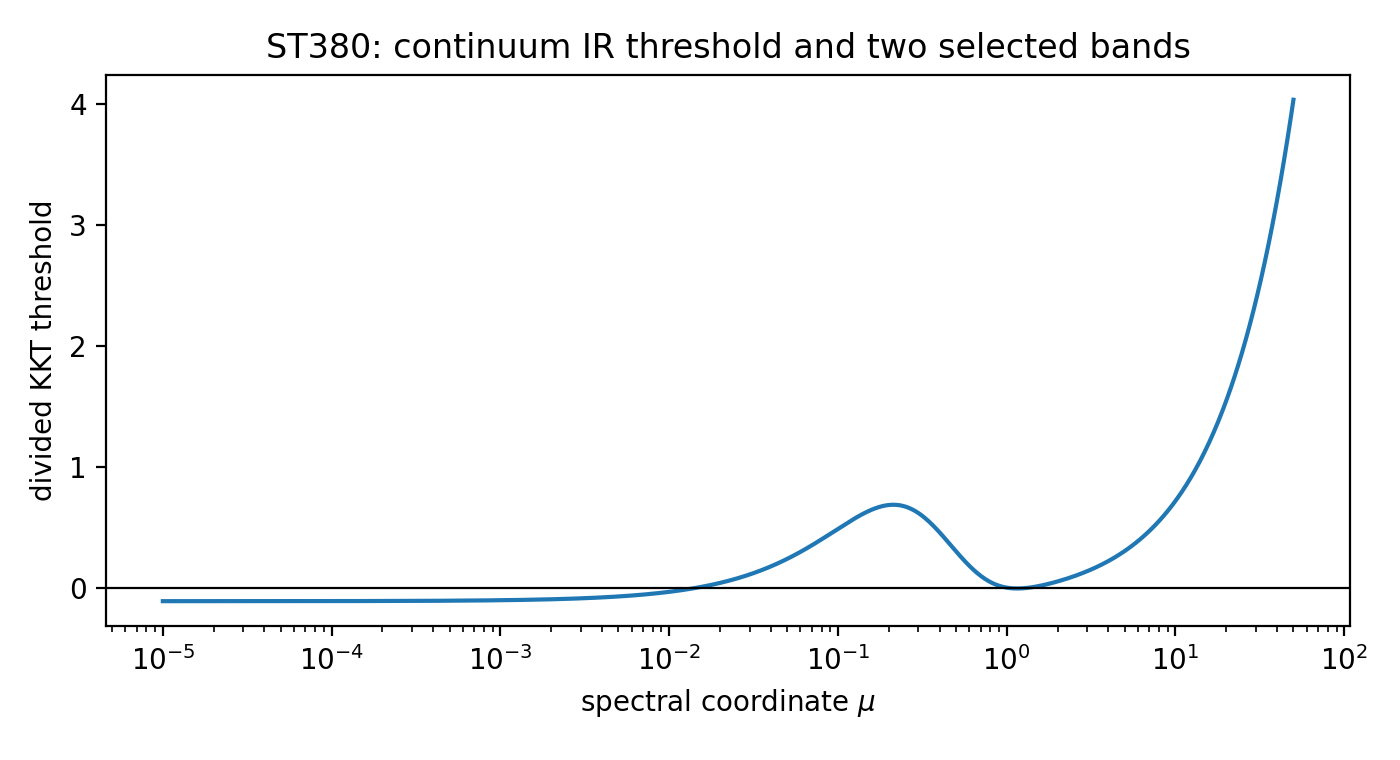
\includegraphics[width=.76\textwidth]{FIN_ST372_ST386_Figures/st380_continuum_ir_threshold.png}
\caption{The certified continuum threshold has exactly three simple roots and two selected bands.}
\end{figure}

This is a real upgrade from a finite grid. It remains a theorem about supplied density,
times, budget, and domain; it is not a strict-derived physical infrared law.

\section{ST381--ST382: Fourier observer geometry and nuisance}

For cyclic convolution experiments $C_p,C_q$, Fourier diagonalization gives
$\widehat{p*r}_k=\widehat p_k\widehat r_k$. If every $\widehat p_k\ne0$, then
\[
\delta(C_p,C_q)=0
\quad\Longleftrightarrow\quad
\operatorname{IDFT}(\widehat q/\widehat p)
\text{ is a probability vector}.
\]
Moreover, $|\widehat v_k|\leq\lVert v\rVert_1=2\operatorname{TV}(v,0)$ and
$|\widehat r_k|\leq1$, yielding
\[
\delta(C_p,C_q)\geq\frac12\max_k
\bigl(|\widehat q_k|-|\widehat p_k|\bigr)_+.
\]
For the ST366 incomparable pair, the bounds are 0.07720 versus the forward LP value 0.2,
and 0.22087 versus the reverse LP value 0.3. They are informative but not generally tight.

ST382 adds calibrated erasure and symmetric label confusion. On the mean-zero sector, the
confusion contrast is $\gamma=|1-12e/11|$. The multinomial error is amplified by the inverse
of the smallest allowed $(1-\ell)\gamma$. Exact operator-norm perturbation supplies an
additional calibration floor. Counts reduce the statistical term but not this floor. The
result assumes declared uncertainty intervals and does not constitute detector calibration.

\section{ST383--ST384: asymptotic compression and dependent clocks}

For the supplied stationary strict-heat Markov source, the entropy rate is
$h=2.605735421009154$ bits/symbol. Per-symbol Fano gives
\[
R(D)\geq\max\{0,h-h_2(D)-D\log_2 11\}.
\]
Time sharing between lossless Markov coding and the constant zero-rate reproduction gives
\[
R(D)\leq h\left(1-\frac{D}{11/12}\right),
\qquad0\leq D\leq11/12.
\]
Thus $R(0)=h$ and $R(11/12)=0$ are proven without extrapolating a block-five computation.

\begin{figure}[H]\centering
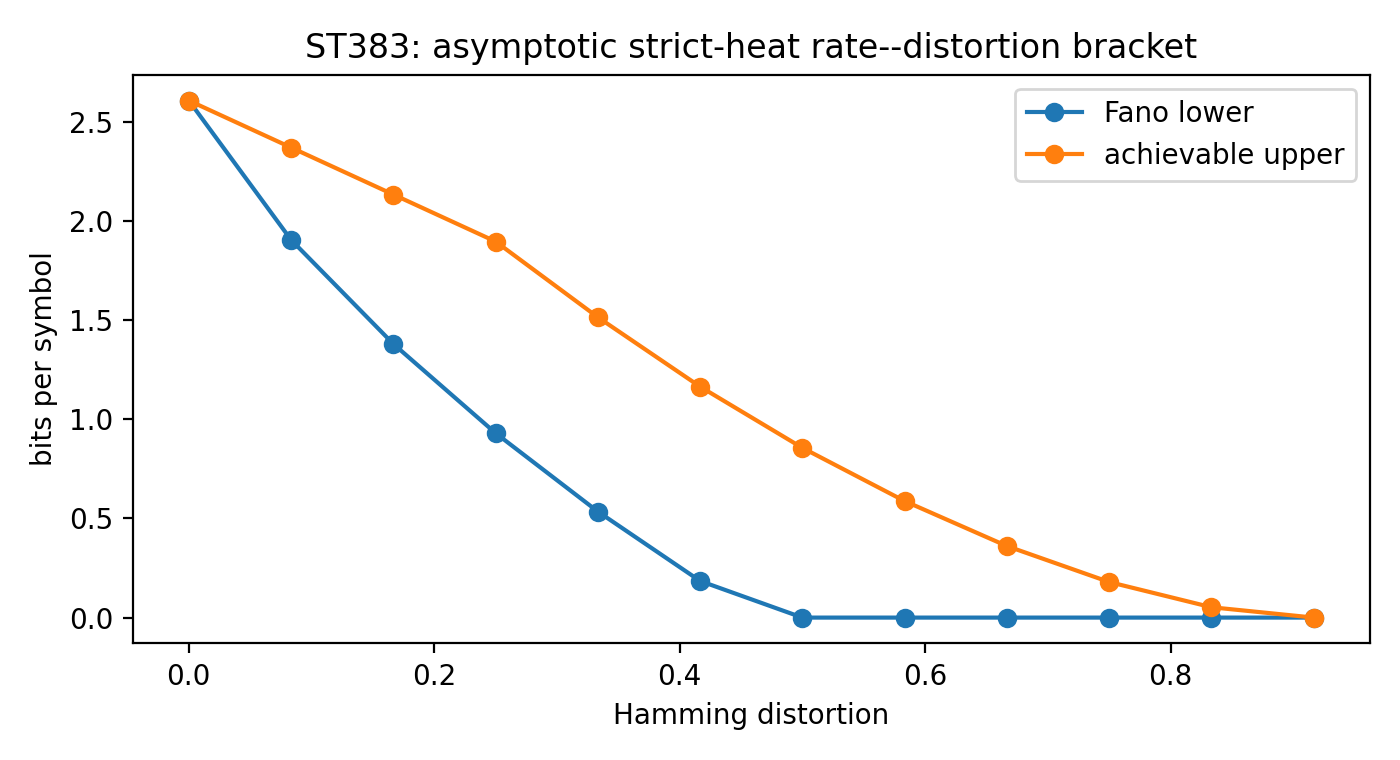
\includegraphics[width=.76\textwidth]{FIN_ST372_ST386_Figures/st383_asymptotic_rate_distortion_bounds.png}
\caption{Rigorous asymptotic bounds; the region between them is not yet the exact function.}
\end{figure}

For relative clocks, suppose centered stationary log-ratio errors satisfy
\[
|\operatorname{Cov}(X_i,X_j)|\leq\sigma^2\rho^{|i-j|}.
\]
Then
\[
\operatorname{Var}\!\left(\sum_{i=1}^{L}X_i\right)
\leq L\sigma^2\frac{1+\rho}{1-\rho}.
\]
Chebyshev preserves square-root-depth concentration; a sharper Gaussian tail applies only
under an additional Gaussian law. Neither covariance decay nor its scale is derived from
the strict operator. No seconds or arrow of time follows.

\section{ST385--ST386: source and evidence stops}

No new typed strict active/selector source packet satisfies the admission pattern. Therefore
closed source and QW-2191 lanes are not replayed. No independently registered raw-event
record is present either. Local mathematics cannot create apparatus, custody,
preregistration, calibration, or empirical events. These are bounded evidence-state stops,
not universal impossibility theorems and not failed experiments.

\section{Synthesis}

This batch materially strengthens three mathematical layers:
\begin{itemize}
\item the global variational problem is now quantitatively localized rather than supported
only by multistart evidence;
\item the nonlinear $D_{12}$ vocabulary is explicit and complete through degree six;
\item the supplied IR design has advanced from a convergent grid pattern to an actual
continuum primal--dual theorem.
\end{itemize}

The results also sharpen the boundary. A nearly closed global value gap is not a proof of
global minimizer identity. A complete invariant basis is not a coefficient or selection law.
A continuum optimum of an imposed design problem does not explain why nature should impose
that density, budget, or those observer times. The operational objects still require
preparation, instrument, environment, calibration, apparatus, and record before they become
testable physics.

Nothing in ST372--ST386 identifies the legacy and strict kernels or transfers the historical
legacy formulas. Nothing breaks the exact strict symmetry or selects orientation without a
new typed source. The present scientific description therefore remains a finite
spectral--variational--informational framework with increasingly strong mathematics, not a
completed physical theory.

\section{Recommended next studies: ST387--ST401}

\begin{longtable}{>{\raggedright\arraybackslash}p{.085\textwidth}>{\raggedright\arraybackslash}p{.17\textwidth}>{\raggedright\arraybackslash}p{.495\textwidth}>{\raggedright\arraybackslash}p{.12\textwidth}}
\toprule Program&Objective&Acceptance criterion&Priority\\\midrule\endhead
ST387&Adaptive slab densification&Insert and certify enough new pseudo-arclength sections to obtain actual chart overlap near the rank event.&High\\
ST388&Interval 2D envelope&Certify the complete $(m,\rho)$ refined envelope and reduce the value gap below $10^{-3}$.&Highest\\
ST389&Twelve-cap interval cover&Cover all concentrated caps, modulo rotations, and isolate every critical box without assuming reflection symmetry.&Highest\\
ST390&Global orbit theorem&Claim uniqueness modulo $D_{12}$ only after ST388/ST389 exclude all asymmetric boxes.&Conditional\\
ST391&Rank-seven global inequality&Construct a mediator-specific replacement for positive-weight collision control, or retain the stop.&Medium\\
ST392&Quartic generators and syzygies&Reduce the 53-element basis to algebra generators and exact relations.&Medium\\
ST393&Sextic coefficient identifiability&Determine which sextic directions are distinguishable from declared observables; do not invent coefficients.&Medium\\
ST394&Quantitative Chernoff gap&Export explicit essential-radius and pressure-derivative error constants over an $s$ interval.&High\\
ST395&Robust continuum IR tube&Interval-certify how roots, bands, and value vary with budget and observer times.&Highest\\
ST396&IR phase diagram&Classify band births/deaths and active-time changes across a bounded supplied parameter cell.&High\\
ST397&Fourier/LP dual equality&Find exact families where the Fourier lower bound attains cyclic deficiency.&Medium\\
ST398&Minimax nuisance lower bound&Match the calibration-floor upper theorem with an adversarial two-point lower bound.&Medium\\
ST399&Markov rate--distortion transfer&Use a tilted transfer operator to narrow or identify the asymptotic $R(D)$ curve.&High\\
ST400&Non-Gaussian dependent clocks&Replace covariance-only Chebyshev by a proved mixing/Bernstein inequality under explicit premises.&Medium\\
ST401&Source/evidence gates&Run only on genuinely new typed source or independently held raw-event packets.&External\\
\bottomrule
\end{longtable}

The preferred local order is ST388 $\rightarrow$ ST389 $\rightarrow$ ST395
$\rightarrow$ ST394. ST387 is a separate validated-continuation track. ST401 must not be
simulated from repository artifacts.

\section{Reproducibility}

The release packet contains the executable program, sixteen live/serialized tests, fifteen
program JSON packets, an aggregate JSON, CSV ledger, three figures, TeX source, PDF, and
SHA-256 manifest. The run uses Python 3, NumPy, SciPy, mpmath interval arithmetic, and
Matplotlib. Modular basis certificates use deterministic mean-zero evaluation points and
prime 1,000,003. All sixteen tests pass.

Internal dependencies are explicit: ST372 consumes the ST298 chain; ST373 consumes the
strict interval weight family; ST375 uses an outward explicit benchmark; ST376 inherits the
ST361 local root; ST379 uses the frozen synthetic filter fixture; ST380 continues the
supplied ST350 design; ST383 uses the conditional strict-heat Markov source. These are
repository results, not independent external validation.

\section{Final verdict}

Release 10.82 produces two genuine upgrades. The global variational obstruction is now a
small, sharply localized residual problem rather than an unconstrained eleven-dimensional
search. Separately, the soft-IR design now has an interval-certified continuum optimum.

Neither upgrade supplies the missing physical principle. The shortest honest next route is
to close the twelve-cap variational cover and to test robustness of the continuum IR
certificate. A source, selector, dimensional calibration, and independent operational
record remain logically separate requirements.

\begin{thebibliography}{9}
\bibitem{CoverThomas} T. M. Cover and J. A. Thomas, \emph{Elements of Information Theory}, Wiley.
\bibitem{Sturmfels} B. Sturmfels, \emph{Algorithms in Invariant Theory}, Springer.
\bibitem{Baladi} V. Baladi, \emph{Positive Transfer Operators and Decay of Correlations}, World Scientific.
\bibitem{LeCam} L. Le Cam and G. L. Yang, \emph{Asymptotics in Statistics}, Springer.
\bibitem{Moore} R. E., R. B. Kearfott, and M. J. Cloud, \emph{Introduction to Interval Analysis}, SIAM.
\end{thebibliography}

\end{document}
